%!TEX TS-program = xelatex
\documentclass[]{friggeri-cv}
\usepackage{afterpage}
\usepackage{graphicx}
\usepackage{hyperref}
\usepackage{color}
\usepackage{pdfpages}
\usepackage{xcolor}
\hypersetup{
    pdftitle={},
    pdfauthor={},
    pdfsubject={},
    pdfkeywords={},
    colorlinks=false,       % no lik border color
   allbordercolors=white    % white border color for all
}
\addbibresource{bibliography.bib}
\RequirePackage{xcolor}
\definecolor{pblue}{HTML}{0395DE}

\begin{document}
\header{Donovan }{Riaño E.}
      {Estudiante Ingeniería en Computación }
      
% Fake text to add separator      
\fcolorbox{white}{gray}{\parbox{\dimexpr\textwidth-2\fboxsep-2\fboxrule}{%
.....
}}

% In the aside, each new line forces a line break
\begin{aside}
  \section{Tel \& Skype}
    +52 55-12-29-16-07
    live:driano7\_1
    ~
  \section{Emails}
    \href{mailto:donovanriano@gmail.com}{\textbf{donovanriano@}\\gmail.com}
    \href{mailto:driano7@outlook.com}{\textbf{driano7@}\\outlook.com}
    ~
  \section{Programación}
    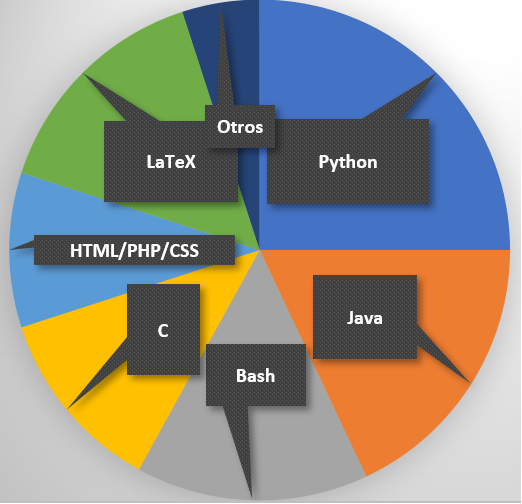
\includegraphics[scale=0.28]{L1.png}
    ~
  \section{OS Preference}
    \textbf{GNU/Linux}
\includegraphics[scale=0.40]{img/4stars.png}
    \textbf{Windows}
\includegraphics[scale=0.40]{img/3stars.png}
    \textbf{MacOS}
\includegraphics[scale=0.40]{img/3stars.png}
    ~
  \section{Lenguajes}
    \textbf{Español}
\includegraphics[scale=0.40]{img/5stars.png}
    \textbf{Inglés}
\includegraphics[scale=0.40]{img/3stars.png}
  ~
  \section{Habilidades Personales}
    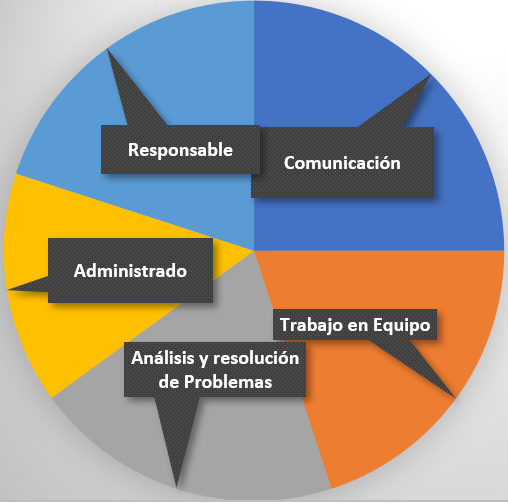
\includegraphics[scale=0.28]{H1.png}
    ~
\end{aside}

\section{Educación}
\begin{entrylist}
\entry
    {2017-Ahora}
    {4to. Semestre Ingeniería en Computación}
    {UNAM, Facultad de Ingeniería}
    {Asignaturas más relevantes: Programación Orientada a Objetos, Inteligencia Artificial, Bases De Datos, Redes de Datos Seguras, Lenguajes Formales y Autómatas.
    %\emph{Title of the Thesis: "A Handoff Algorithm based on Link Quality Prediction for Mass Transit Wireless Mesh Networks"      .}\\
    %\emph{Relators: Prof. Enzo Mingozzi, Ing. Carlo Vallati, Prof. Luciano Lenzini.}\\
    }
\entry
    {Invierno 2018}
    {Curso extracurricular}
    {Anexo de Ingeniería, UNAM, CDMX}
    {La Integral, Métodos de Integración y Aplicaciones\\
    Finalidad del curso: aplicaciones de las Integrales, 15 Horas.}

\entry
    {Verano 2019}
    {Curso extracurricular}
    {Anexo de Ingeniería, UNAM, CDMX}
    {Python \& Machine Learning Avanzado\\
    Finalidad del curso: ejemplos, implementaciones y usos de redes neuronales artificiales en la herramienta Colab, 10 horas.}

\end{entrylist}

\section{Experiencia Laboral}
\begin{entrylist}
  \entry
    {Verano 2018}
    {CAE IECM}
    {Aniceto Ortega 917, Benito Juárez, CDMX}
    {Capacitador Asistente Electoral elecciones 2018.\\}
  
\end{entrylist}


%\section{Certifications}
%\begin{entrylist}
%  \entry
%    {02/2013}
%    {Intro to Computer Science}
%    {Udacity. E-learning}
%    {\emph{Building a Python Search Engine}}
%\end{entrylist}

\section{Futuras Publicaciones}
Riaño D.\\
\textbf{Tratamiento de Expresiones Regulares en la Privacidad de Navegadores Web}\\
\emph{CONISOFT-2019 , Facultad de Ingeniería, UNAM, CDMX, Octubre 23-25, 2019.}
\\
\section{Otra Información}

\emph{Procesador de Textos \LaTeX. \\ }
\emph{Nociones: Bases de Datos en PHP myAdmin, Interfaces Gráficas en Java, Optical Character Recognition (OCR) con Tesseract y OpenCV en Python, API Speech Recognition de Google en Python. \\}
\emph{Software: Word, Excel, PowerPoint, LibreOffice, SublimeText, Brackets, Visual Studio, Bash Linux.\\ }
%\emph{ }
\\
\begin{flushleft}
\emph{Julio 1, 2019}
\end{flushleft}
\begin{flushright}
\emph{Donovan Riaño Enriquez}
\end{flushright}

\clearpage


\includepdf[pages={1}]{Comp.pdf} 
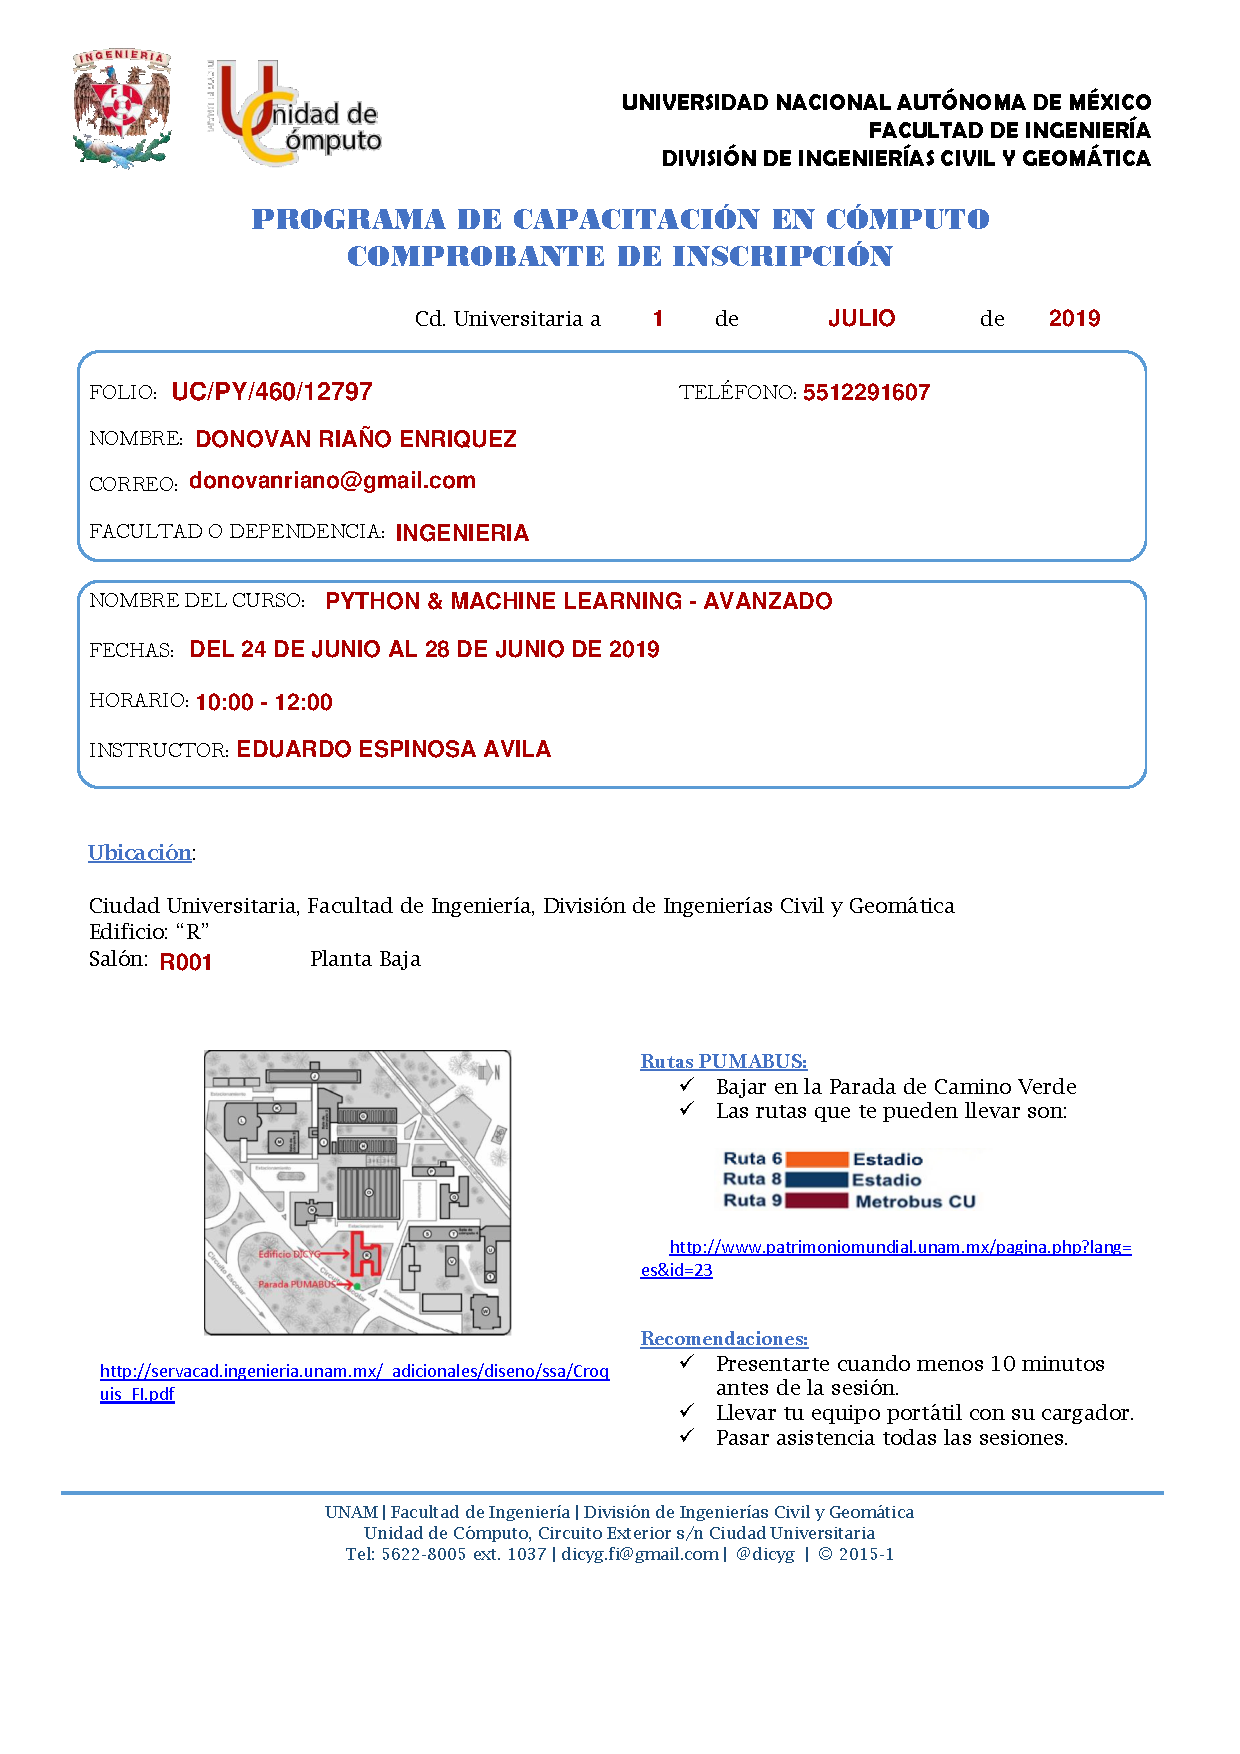
\includepdf[pages={1}]{machine.pdf} 
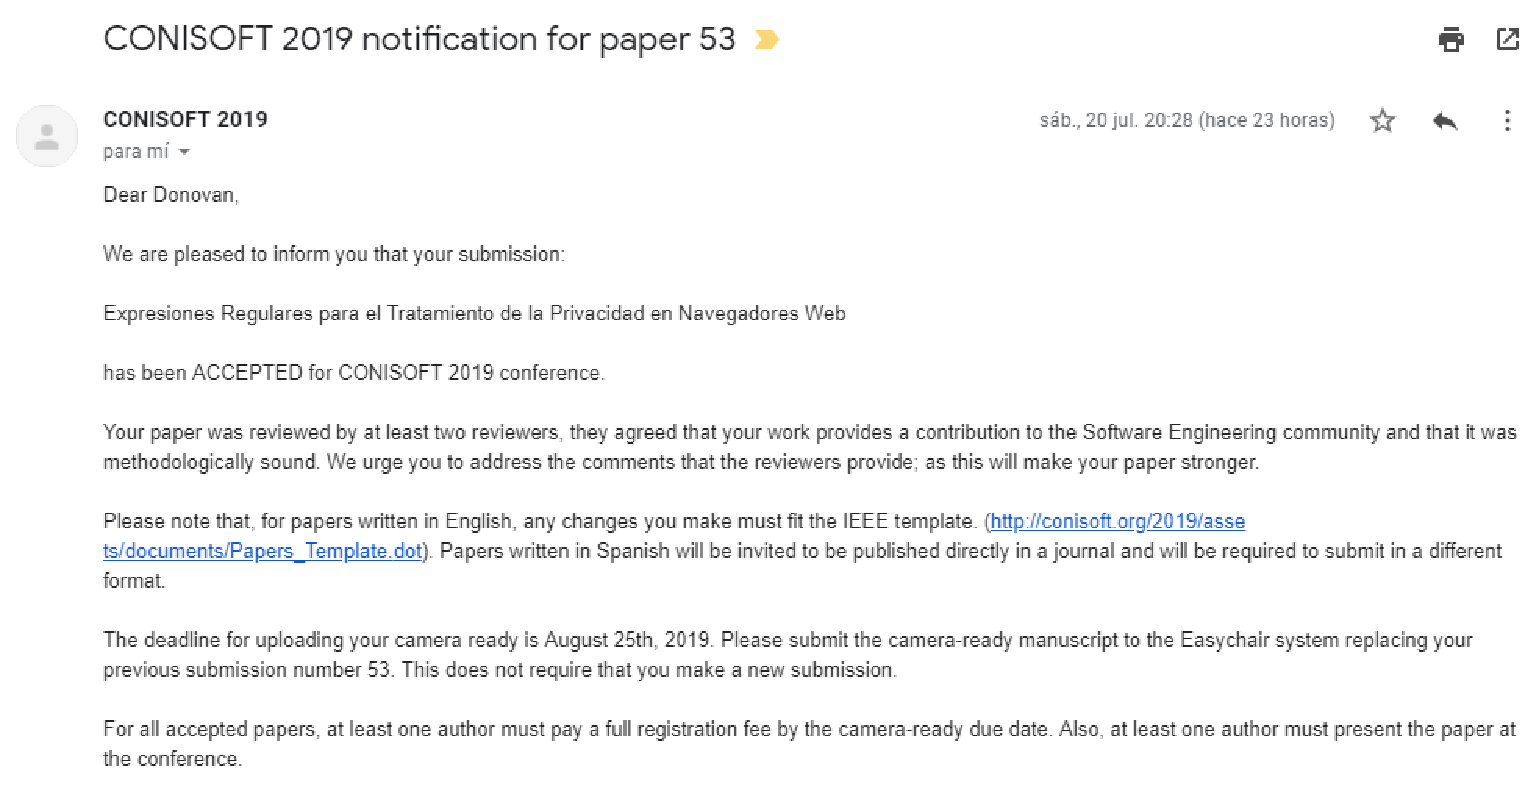
\includepdf[pages={1}]{aceptacion.pdf} 
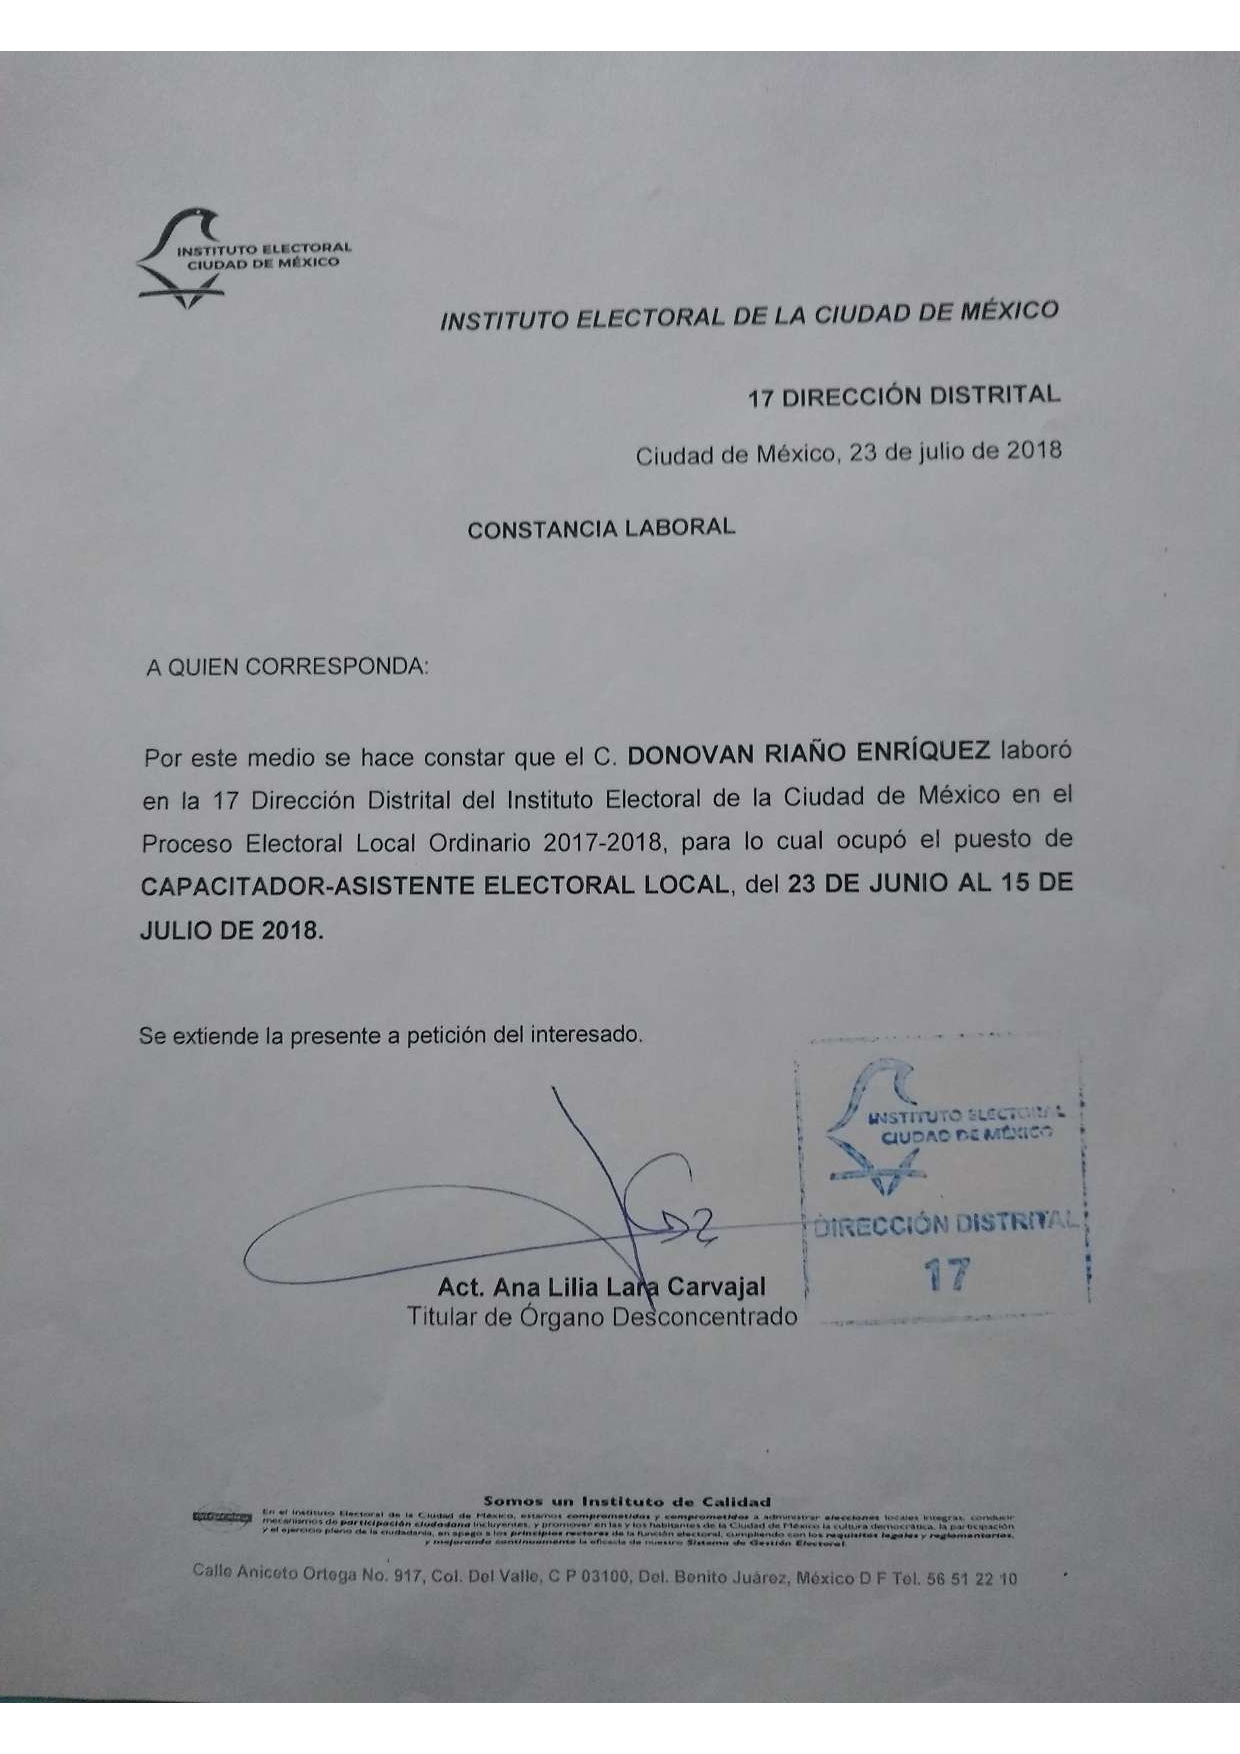
\includepdf[pages={1}]{Iecm.pdf} 


%%% This piece of code has been commented by Karol Kozioł due to biblatex errors. 
% 
%\printbibsection{article}{article in peer-reviewed journal}
%\begin{refsection}
%  \nocite{*}
%  \printbibliography[sorting=chronological, type=inproceedings, title={international peer-reviewed conferences/proceedings}, notkeyword={france}, heading=subbibliography]
%\end{refsection}
%\begin{refsection}
%  \nocite{*}
%  \printbibliography[sorting=chronological, type=inproceedings, title={local peer-reviewed conferences/proceedings}, keyword={france}, heading=subbibliography]
%\end{refsection}
%\printbibsection{misc}{other publications}
%\printbibsection{report}{research reports}

\end{document}
